\chapter{Proof fields, closure, and executable certificates}\label{ch:prooffields}

A reasoning archive contains more than its final proofs. It may retain alternative derivations, conjectures, unsuccessful proposals, and observations that later become obsolete. A checker must know which of those records it is permitted to use. Otherwise an archive that is useful for discovery can become an unsound source of premises.

Proof-Path Theory supplies a finite distinction between the surrounding field and the certified derivation. This chapter admits its closure and trace-checking results in a self-contained form. It does not identify acceptance of a data structure with truth of an arbitrary sentence attached to that structure.

\section{A finite field with explicitly admitted rules}
Let $V=\{0,\ldots,n-1\}$ be a finite set of claim addresses. Let $A\subseteq V$ be admitted leaves, $S\subseteq V$ positive observations, and $N\subseteq V$ forbidden consequences. These sets need not be disjoint. A finite rule list $R$ has rows
\[
 r_j=(P_j,c_j),\qquad P_j\subseteq V,\quad c_j\in V.
\]
Only admitted rules are included. Identical rows may occupy different addresses. A conjectural rule elsewhere in the discovery archive is not admitted merely because it has a convenient conclusion.

A model of the field is a set $B\subseteq V$ containing $A$ and satisfying every implication $P_j\subseteq B\Rightarrow c_j\in B$. A protected extension also contains $S$ and avoids $N$. Define
\[
 C_0=A\cup S,\qquad
 C_{k+1}=C_k\cup\{c_j:P_j\subseteq C_k\}.
\]
The terms increase and lie in $V$, so the sequence stabilizes. Write $C$ for its stable value.

\begin{proposition}[The least seeded model]\label{r:field-closure}
The set $C$ is the least model containing $S$. There are at most $n-|A\cup S|$ strict expansion rounds. A protected extension exists if and only if $C\cap N=\varnothing$.
\end{proposition}
\begin{proof}
At a fixed point every enabled rule has its conclusion in $C$, so $C$ is a model containing the seeds. If $B$ is any other model containing $S$, induction gives $C_k\subseteq B$: the seeds lie in $B$, and every rule enabled on $C_k$ has its conclusion in $B$. Hence $C\subseteq B$. Each strict expansion adds at least one of the finitely many nonseed nodes, giving the bound. If $C$ avoids $N$, it is itself a protected extension. If it meets $N$, every seeded model contains that forbidden node, so no protected extension exists.
\end{proof}

A cycle does not create a seed. With rules $u\to v$ and $v\to u$ and no admitted leaves or observations, the least model is empty. The set $\{u,v\}$ is closed, but its members have no derivation from the empty seed. This is why closedness alone is not an adequate proof certificate.

\section{Replay checks a finite causal sequence}
A trace $\sigma=(j_1,\ldots,j_m)$ lists rule addresses. Start from $K_0=A\cup S$. At each step, reject an unknown rule address or a rule whose premises are not all in the current known set. Otherwise adjoin its conclusion. \emph{Strict replay} also rejects a conclusion already known. \emph{Causal replay} allows it.

The distinction concerns the certificate's contract, not the truth of a repeated conclusion. Strict replay records a sequence of new insertions. Causal replay permits reuse of an existing derivation after stronger observations have already supplied one of its intermediate nodes.

\begin{theorem}[Replay is sound and compositional]\label{r:field-replay}
If replay accepts a trace from a set $K\subseteq C$ and returns $K'$, then
\[
 K\subseteq K'\subseteq C.
\]
For either fixed replay mode, replay of a concatenated trace is replay of its first part followed by replay of its second part from the returned set. Failure in either part is failure of the concatenated replay.
\end{theorem}
\begin{proof}
The empty trace changes nothing. At a successful next step, all premises of an admitted rule already lie in $C$. Closedness of $C$ places its conclusion in $C$. Adjoining it preserves the old known set. Induction proves the inclusions. A strict novelty test can reject a step, but does not alter this reasoning for an accepted step.

For concatenation, induct on the first trace. Both computations inspect the same first address, the same current set, and the same enabling and novelty conditions. A rejection ends both computations. A successful step produces identical new sets, after which the induction hypothesis applies.
\end{proof}

\begin{theorem}[Replay and saturation identify exact closure]\label{r:field-exact}
A complete-closure certificate consists of a strict trace and a reported set $B$. Accept it only when replay from $A\cup S$ succeeds with output $B$ and $B$ satisfies every admitted rule. Acceptance implies $B=C$.
\end{theorem}
\begin{proof}
Replay soundness gives $B\subseteq C$. Its extensivity ensures that $B$ contains both seed sets. The saturation check makes $B$ a seeded model, so leastness gives $C\subseteq B$. The two inclusions prove equality.
\end{proof}

The tests serve different purposes. Replay prevents unsupported extra nodes. Saturation prevents omission of a consequence whose rule has not yet been used. Neither test subsumes the other.

\section{A complete negative answer has a witness}
An obstruction certificate contains a forbidden target $v\in N$ and a causal trace deriving $v$ from $A\cup S$.

\begin{theorem}[Finite obstruction witnesses are sound and complete]\label{r:field-obstruction}
An accepted obstruction certificate exists exactly when no protected extension exists. No acyclicity assumption on the rule graph is required.
\end{theorem}
\begin{proof}
An accepted certificate derives a node of $C\cap N$, so Proposition~\ref{r:field-closure} excludes a protected extension.

Conversely, if there is no extension, choose $v\in C\cap N$. Every node in $C$ is reached at a finite stage. Starting with the seeds, process the rules that add the nodes of each successive stage, appending a rule only when its conclusion is not yet known. All its premises belong to an earlier stage and are already known. This yields a finite strict trace reaching the whole closure, and in particular $v$. Its prefix ending when $v$ is first present is also accepted in causal mode. If $v$ is a seed, the empty trace suffices. Cycles cause no difficulty because only rules with already known premises are applied.
\end{proof}

The argument constructs some witness, not a shortest one. Nor does it prove that every implementation of a witness producer terminates or faithfully indexes its source document. A complete result format can require both exact closure and a feasibility flag. A bare negative witness needs only its own replay and forbidden-target check.

\section{A worked four-node certificate}
Let $V=\{0,1,2,3\}$, $A=\{0\}$, $S=\varnothing$, and let the two rules be $0\to1$ and $1\to2$. The exact closure is $\{0,1,2\}$.

The trace containing only the first rule is a valid partial derivation of $\{0,1\}$, but it fails saturation. The set $\{0,1,2,3\}$ is saturated, but node $3$ cannot be produced by replay. The trace of both rules and the exact three-node set pass both tests.

\begin{figure}[htbp]\centering
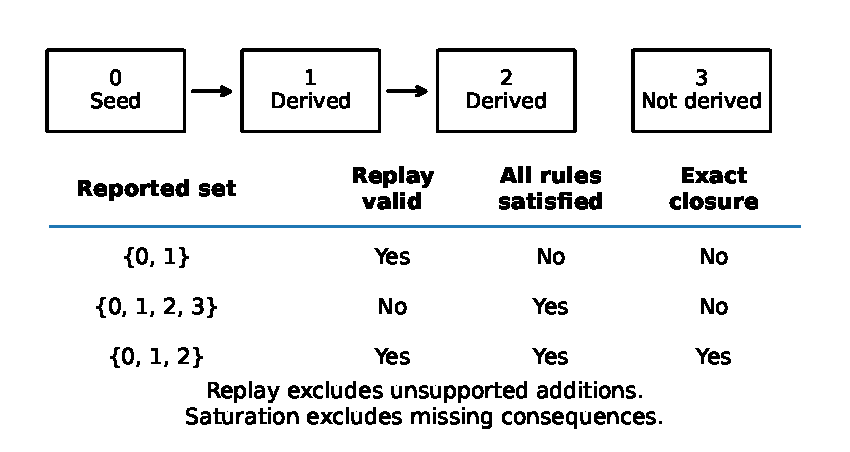
\includegraphics[width=.94\linewidth]{figures/closure_contract.pdf}
\caption{Replay and saturation certify opposite inclusions. A partial derivation omits a consequence. A closed superset can contain an unsupported node. Their conjunction identifies the least seeded model.}\label{fig:closure-contract}
\end{figure}

With forbidden set $N=\{3\}$, the exact closure is a positive feasibility certificate. With $N=\{2\}$, the same closure and the trace to node $2$ certify infeasibility. The request changed, even though the derivation did not. A receiving checker must therefore be given the intended request separately from the producer's proposed answer.

\section{Logical interpretation is an additional map}
Let $\mu(v)$ be the proposition represented by claim address $v$. Suppose every admitted leaf and positive observation is true under $\mu$, and each admitted rule satisfies
\[
 \left(\bigwedge_{p\in P_j}\mu(p)\right)\Longrightarrow\mu(c_j).
\]
Then every node in $C$ is true under $\mu$. Indeed, induction over the closure stages propagates truth from the seeds through the admitted implications.

The finite checker proves derivability relative to those inputs. It does not establish the truth of an empirical observation merely because that observation is placed in $S$. A node excluded by a protected request is likewise not necessarily a logically false proposition. Its appearance shows incompatibility with that request, whose meaning must be stated separately.

\section{The serialization and implementation boundary}
An exchange format must distinguish a problem from its proposed certificate, preserve rule addresses, and reject malformed node identifiers. In Python, for example, a Boolean passes a broad integer-instance test. An address decoder that intends exact integer tokens must exclude that case explicitly. Parsing, range checking, replay, saturation, and interpretation are separate operations.

The Proof-Path Theory source supplies typed problem and certificate records, proved encoder/decoder round trips, an executable Lean replay function, and an accepted-answer theorem at the Lean JSON syntax-tree boundary. Its text parser, file operations, Python implementation, and adapter from named source claims remain separate assurance layers. This chapter uses the finite closure and replay statements, not a blanket verification claim for that entire path.

\source{Proof-Path Theory [PPT], ``Executable certificates for the declared closure,'' ``Finite witnesses for forbidden consequences,'' and ``Typed exchange and the boundary of serialization.'' The selected source statements are \texttt{res:trace:replay}, \texttt{res:trace:least}, \texttt{res:trace:complete}, and \texttt{res:trace:verdict}. Their original formal concordance is preserved with the source excerpt. The present notation and proofs were reviewed as a restatement, not recompiled into a new Lean development.}

\section{Where proof checking enters the reasoning calculus}
The machine-reasoning chain now has a concrete certificate interface. A discovery process can propose a finite derivation without becoming the authority on its validity. The checker verifies the derivation against a fixed problem. A revision can change the problem or its admitted rules, in which case the dependency and migration conditions must be checked again. Reusing the same bytes does not establish that the old certificate answers the new question.
